\documentclass[a4paper, 12pt]{article}
\usepackage{listings} 
\usepackage{xcolor}
\usepackage{mdframed}
\usepackage{graphicx}
\usepackage{pgfplots}
\usepackage{float}
\usepackage{mathtools}
\usepackage[margin=1.00in]{geometry}
\DeclarePairedDelimiter\ceil{\lceil}{\rceil}
\DeclarePairedDelimiter\floor{\lfloor}{\rfloor}

\definecolor{code-gray}{gray}{0.93}
\begin{document}
\title{ECE 341 - Lab \#9}
\author{Collin Heist}
\date{\today}
\maketitle
\pagenumbering{roman}
\tableofcontents
\lstlistoflistings
\newpage
\pagenumbering{arabic}

\section{Introduction}
The purpose of this lab is to learn how to implement a basic PWM signal using the on-board output compare module. We'll be using this PWM signal to control the speed of a motor connected to the board. Rather than the previous  motor we've interacted with, which required stepping through a finite state machine of motor states in the outputs, the motor for this week takes a PWM signal and that (roughly) equates to how much energy is being delivered to the motor. By varying the width of the pulse, the speed changes correspondingly. 

The only new peripheral for this week is the output compare module. This works through two registers that we, the user, can load digital values into. These digital values are then compared to the digital value of the corresponding timer's attached register. By adjusting both the timer's period register, and the value loaded into those two output compare registers, the PWM signal's width will drop from logical high to low at different times. For example, if the timer's period register is set to 4, and the value inside the output compare register was set to 1, this would correspond to the output only staying high during the two ticks of the clock where the value is less than or equal to that 1 (so cycle 0, and cycle 1). 

This concept can be used to convert 'percentages' that correspond to duty cycles to values loaded into those compare registers. For example, a 10\% duty cycle would require loading 0.1 times the period register for the corresponding timer.

\section{Implementation}
The first function I wrote for my PWM library was the initialization function. This initializes timer 2, the timer associated with the output compare (PWM) module, as well as the PWM module itself. This code is shown in Listing~\ref{lst:pwmInit}.

	\begin{mdframed}[backgroundcolor=code-gray, roundcorner=10pt,
								innerleftmargin=5, innertopmargin=5, innerbottommargin=5]	
	\begin{lstlisting}[language=C, caption=PWM and Timer 2 Initialization, tabsize=2, label={lst:pwmInit}]
	unsigned int init_pwm(unsigned int duty_cycle,
		unsigned int pwm_freq) {
		
		t2_tick = T2_CLOCK_RATE / pwm_freq;
		if (t2_tick > 2^16)
			return 1;
		OpenTimer2(T2_ON | T2_SOURCE_INT | T2_PS_1_1, t2_tick - 1);
		mT2SetIntPriority(2);
		mT2SetIntSubPriority(1);
		mT2IntEnable(1);

		if (duty_cycle > 100)
			return 1;
		unsigned int start_val = duty_cycle * (t2_tick - 1);
		OpenOC3(OC_ON | OC_TIMER_MODE16 |
			OC_TIMER2_SRC | OC_PWM_FAULT_PIN_DISABLE,
			start_val, start_val);

		return 0;
	}
	\end{lstlisting}
	\end{mdframed}
	
For a given starting PWM duty cycle (a percentage between 0\% and 100\%), and a PWM frequency (how many times the output compare module is asserted each second), this function initializes timer 2 to the necessary value, turns on its interrupt, and then starts the output compare module. The variable \textbf{t2\_tick} is defined as a global variable inside the header file \textbf{pwm.h}. 

As per the lab's instructions, invalid clock PWM frequencies or duty cycles result in a return of 1, meaning an error occured. Otherwise, a 0 is returned (indicating no error).

The only other function I needed to write was the code to allow the user to change the PWM cycle accordingly. For easier use, the user provides only a percentage (just like in Listing~\ref{lst:pwmInit}) that corresponds to a duty cycle. This value is then 'scaled' between 0 and the current period register for timer 2. This function is shown in Listing~\ref{lst:pwmSet}

	\begin{mdframed}[backgroundcolor=code-gray, roundcorner=10pt,
								innerleftmargin=5, innertopmargin=5, innerbottommargin=5]	
	\begin{lstlisting}[language=C, caption=PWM Duty Cycle Set Function, tabsize=2, label={lst:pwmSet}]
	unsigned int set_pwm(unsigned int duty_cycle) {
		if (duty_cycle > 100)
			return 1;

		SetDCOC3PWM((float) duty_cycle / 100.0 * (t2_tick - 1));

		return 0;
	}
	\end{lstlisting}
	\end{mdframed}
	
A similar return scheme is used for this, if a non-valid duty cycle is given to the function (i.e. greater than 100\%, as it is an unsigned integer, so no negatives occur) then the function returns a non-zero value (1). Provided a valid percentage is given, then that value is loaded into the shadow register of the output compare module after scaling it between 0 and the period register for timer 2 minus 1. The reason for subtracting one is because the timer counts up to \textbf{t2\_tick}, which since it starts at 0, takes \textbf{t2\_tick} + 1 clock cycles. Thus, a subtraction of one is necessary. Afterwards, a 0 is returned.

There is \textit{technically} one more piece of code inside the \textbf{pwm.c} file, but it is just the timer 2 \textbf{ISR} used in the previous labs, so it is not shown here. This could have been put inside the other files, but since the timer is initialized inside this file, it is logically consistent to keep its interrupt routine here as well. The header file is very short, but is shown in Listing~\ref{lst:pwmheader}

	\begin{mdframed}[backgroundcolor=code-gray, roundcorner=10pt,
								innerleftmargin=5, innertopmargin=5, innerbottommargin=5]	
	\begin{lstlisting}[language=C, caption=PWM Header File, tabsize=2, label={lst:pwmheader}]
	#ifndef __PWM_H__
		#define __PWM_H__

		#define T2_PRESCALE			1
		#define T2_CLOCK_RATE		(FPB / T2_PRESCALE)
	#endif

	// Function prototypes
	...
	\end{lstlisting}
	\end{mdframed}
	
Should a different prescale value be used, that could be changed here. Otherwise, the only important thing is the clock rate, which is defined as the peripheral bus clock divided by the prescale value. In this case, this is a constant 10 MHz, but could feasibly be changed for higher frequency PWM outputs.

With the PWM library code finished, the next step was the main file which implemented said library. To begin, the system initialization function:

	\begin{mdframed}[backgroundcolor=code-gray, roundcorner=10pt,
								innerleftmargin=5, innertopmargin=5, innerbottommargin=5]	
	\begin{lstlisting}[language=C, caption=System Initialization, tabsize=2, label={lst:sysinit}]
	void system_init() {
		Cerebot_mx7cK_setup();
		init_LCD();
		reset_clear_LCD();
		PORTSetPinsDigitalOut(IOPORT_B, SM_LEDS);
		PORTSetPinsDigitalOut(IOPORT_D, BIT_1);
		PORTSetPinsDigitalIn(IOPORT_D, BIT_3 | BIT_12);
		LATBCLR = SM_LEDS;
		LATDCLR = BIT_1; 
	
		mCNOpen(CN_ON, (CN8_ENABLE | CN9_ENABLE), 0);
		mCNSetIntPriority(1);
		mCNSetIntSubPriority(0);
		unsigned int x = PORTReadBits(IOPORT_G, BTN1 | BTN2);
		mCNClearIntFlag();
		mCNIntEnable(1);

		init_pwm(40, 1000);

		INTEnableSystemMultiVectoredInt();
	}
	\end{lstlisting}
	\end{mdframed}
	
As usual, the cerebot is first setup, then I initialize and then clear the LCD, declare the instrumentation LED's as outputs, then the motor direction pin as an output. This is the actual pin we'll be toggling using the output compare module. The next line of input puts is not used in this lab. I initialize the change notice interrupts for buttons 1 and 2, as usual,and  initiate a dummy read to avoid immediately triggering them. Finally, my PWM initialization function is called with a starting duty cycle of 40\%, and a frequency of 1000 Hz (as given in the lab instructions). Interrupts are then globally enabled. As stated before, timer 2 is not initialized in this code because the \textbf{init\_pwm()} function takes care of that for me.

Since we are no longer using a FSM to control a motor, and instead each combination of buttons corresponds to a different speed for the motor, the \textbf{decode\_buttons()} function was changed to the following: 

	\begin{mdframed}[backgroundcolor=code-gray, roundcorner=10pt,
								innerleftmargin=5, innertopmargin=5, innerbottommargin=5]	
	\begin{lstlisting}[language=C, caption=Decode Buttons, tabsize=2, label={lst:btndecode}]
	unsigned int decode_buttons(unsigned int portG_state) {
		unsigned int btns = portG_state >> 6;
		unsigned int cases[] = {40, 65, 80, 95};

		return cases[btns];
	}
	\end{lstlisting}
	\end{mdframed}
	
This is a very short and straightforward function. The lab outlines different duty cycles for each button combination, and the corresponding duty cycle is simply returned based on the state of the buttons.

Next is the interrupt routine for the button presses. A lot happens here, as that's the only I/O for the system in this lab. The code is shown in Listing~\ref{lst:cnisr}

\begin{mdframed}[backgroundcolor=code-gray, roundcorner=10pt,
								innerleftmargin=5, innertopmargin=5, innerbottommargin=5]	
	\begin{lstlisting}[language=C, caption=Change Notice ISR, tabsize=2, label={lst:cnisr}]
	void __ISR(_CHANGE_NOTICE_VECTOR, IPL1) CNIntHandler(void) {
		LATBINV = LEDC;
		sw_ms_delay(20);
		unsigned int buttons = read_buttons();
		pwm_cycle = decode_buttons(buttons);
		set_pwm(pwm_cycle);

		char pwm_str[8] = {'\0'};
		sprintf(pwm_str, "%u\%%\n", pwm_cycle);
	
		char lcd_str[50] = "PWM Cycle: ";
		strcat(lcd_str, pwm_str);

		char dash_str[20] = {'\0'};
		unsigned int num_dashes = (float) pwm_cycle / (100.0 / 16.0);
		unsigned int i;
		for (i = 0; i < num_dashes; i++)
			dash_str[i] = '-';

		strcat(lcd_str, dash_str);

		reset_clear_LCD();
		put_string_LCD(lcd_str);

		LATBINV = LEDC;
		mCNClearIntFlag();
	}
	\end{lstlisting}
	\end{mdframed}
	
For debugging, LED C is toggled at the beginning and end of this ISR. After a 20ms software debounce period, the buttons are read (using the functions created in previous labs), and then decoded. The decoding function was shown in Listing~\ref{lst:btndecode}. The returned duty cycle is then send to the PWM library's \textbf{set\_pwm()} function which loads the correct value into the output compare registers. The following sections of code are simply string manipulation to output the current duty cycle on the LCD (as well as a variable number of dashes corresponding to the width of the pulse). The LCD is then cleared, and the cycle is displayed.

With that, the program is essentially completed. The main function is left blank, except for the system initialization, and then an empty infinite while loop.

\section{Testing and Verification}
As usual, to test my code for this lab, the LCD was a nice indicator of whether or not the button presses were being decoded correctly. Since I was not \textit{running} the motor throughout this lab, as it is very loud, I looked at the LED pulses on the oscilloscope for verification. Below (Figure~\ref{fig:scope6}) is the one millisecond period of the timer:

\begin{figure}[H]
\centering
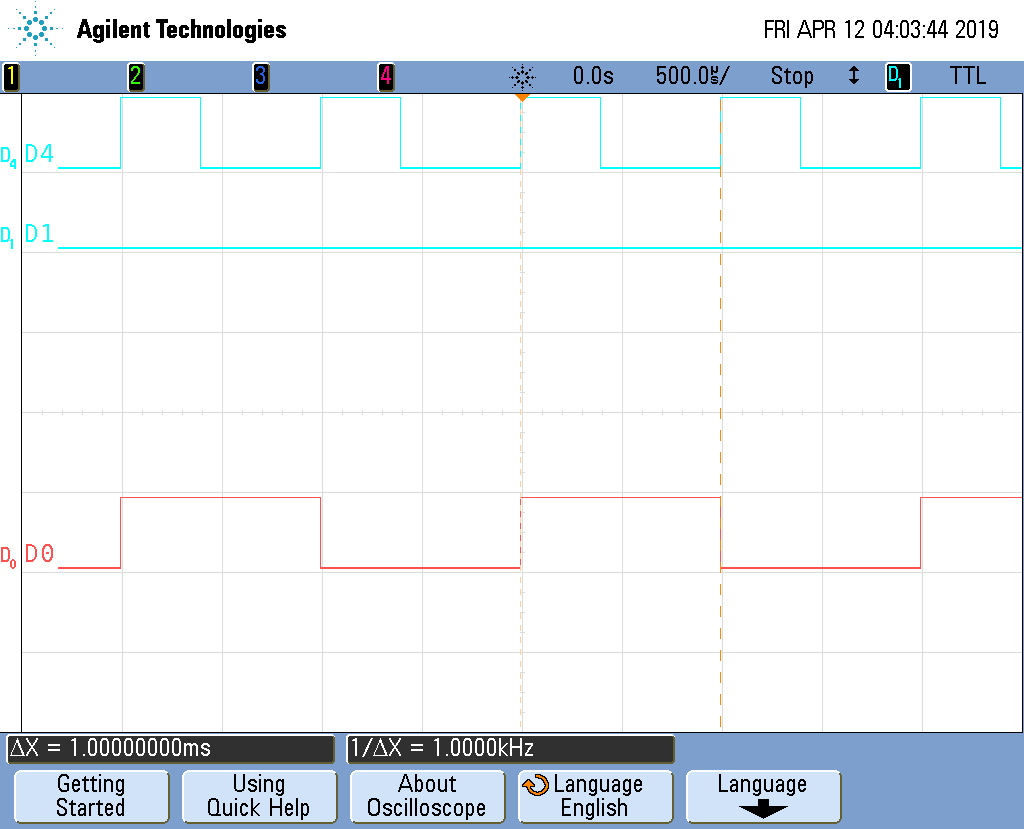
\includegraphics[width=.8\textwidth]{scope_6.png}
\caption{1ms Timer 2 Period}
\label{fig:scope6}
\end{figure}

I also took captures of the CN ISR, which takes quite a while because of the debounce as well as the LCD interfacing which is not very quick. The different duty cycles are also attached as Figures~\ref{fig:scope7}, ~\ref{fig:scope9}, ~\ref{fig:scope10}, and~\ref{fig:scope11}.

\begin{figure}[H]
\centering
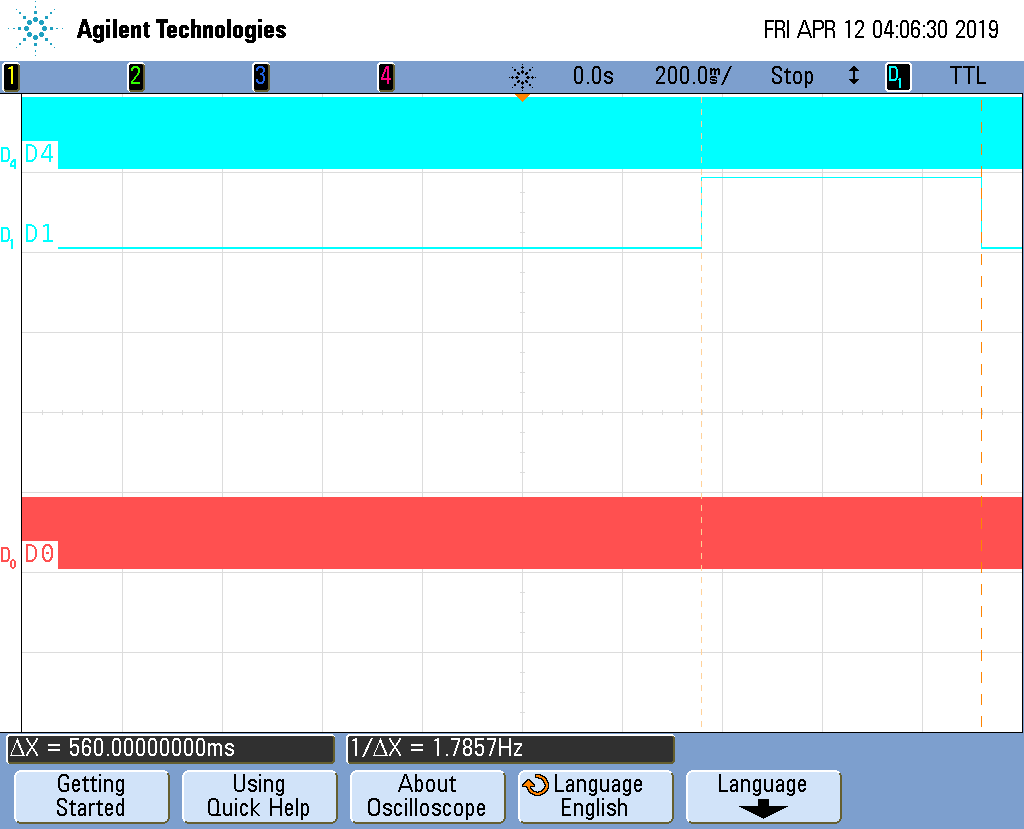
\includegraphics[width=.8\textwidth]{scope_8.png}
\caption{CN Interrupt Width}
\label{fig:scope8}
\end{figure}

\begin{figure}[H]
\centering
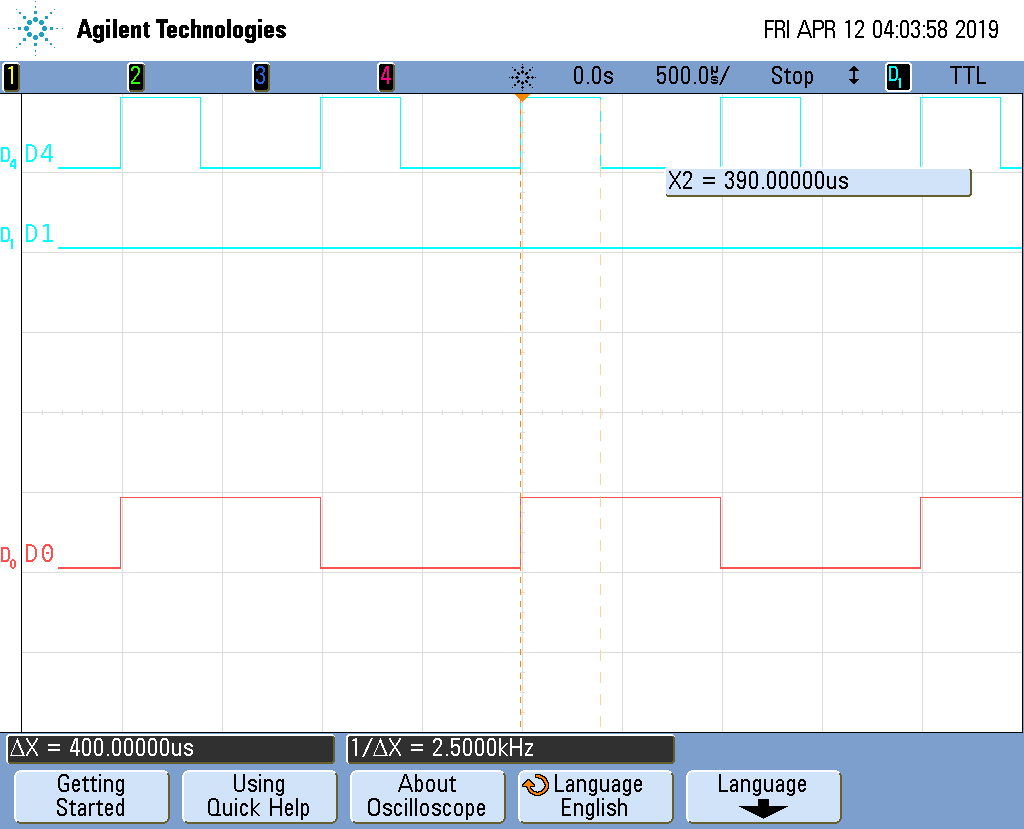
\includegraphics[width=.8\textwidth]{scope_7.png}
\caption{40\% Duty Cycle}
\label{fig:scope7}
\end{figure}

\begin{figure}[H]
\centering
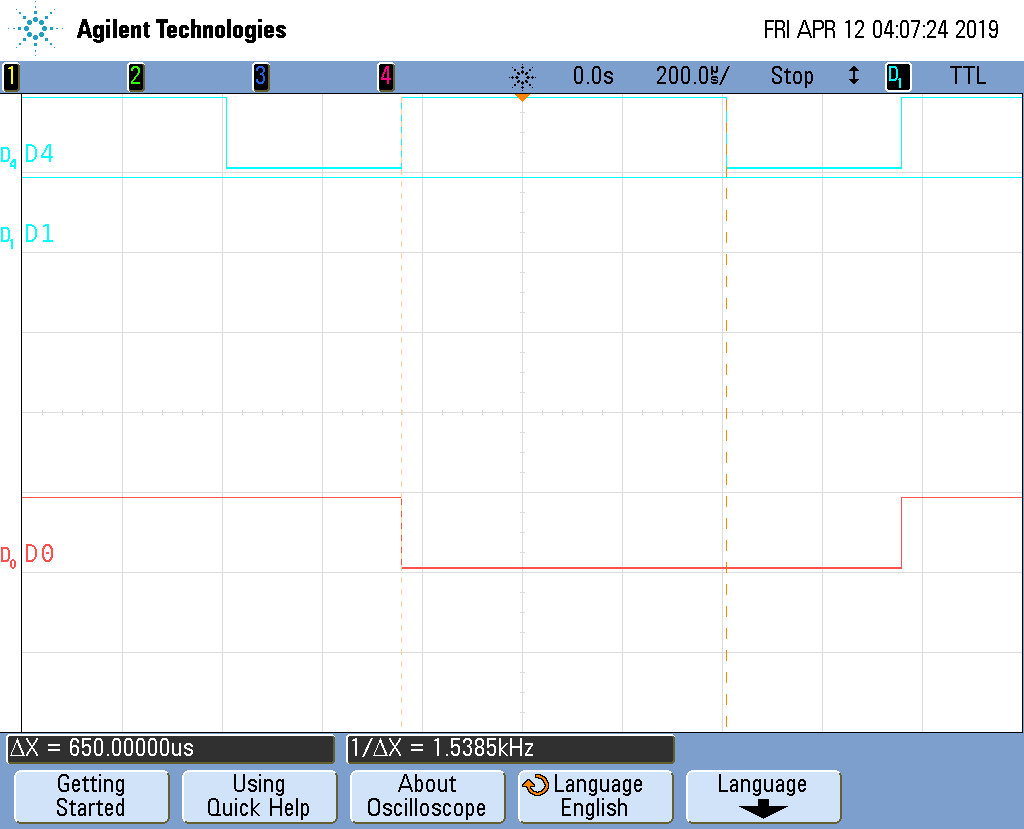
\includegraphics[width=.8\textwidth]{scope_9.png}
\caption{65\% Duty Cycle}
\label{fig:scope9}
\end{figure}

\begin{figure}[H]
\centering
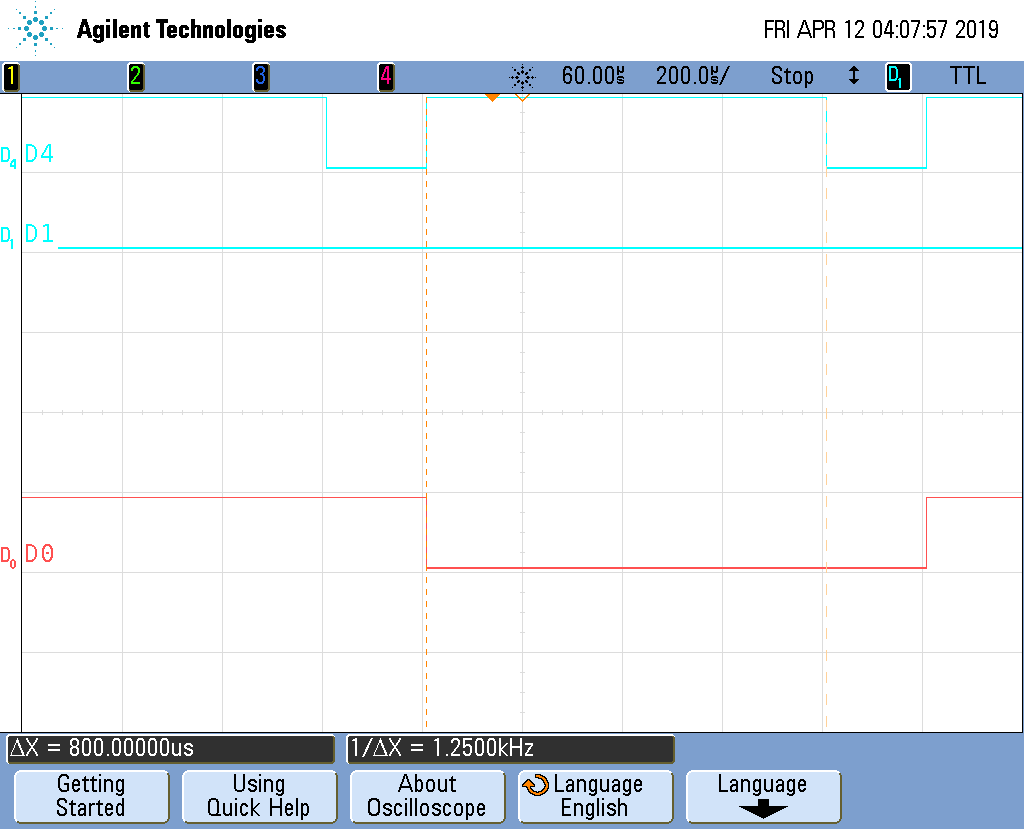
\includegraphics[width=.8\textwidth]{scope_10.png}
\caption{80\% Duty Cycle}
\label{fig:scope10}
\end{figure}

\begin{figure}[H]
\centering
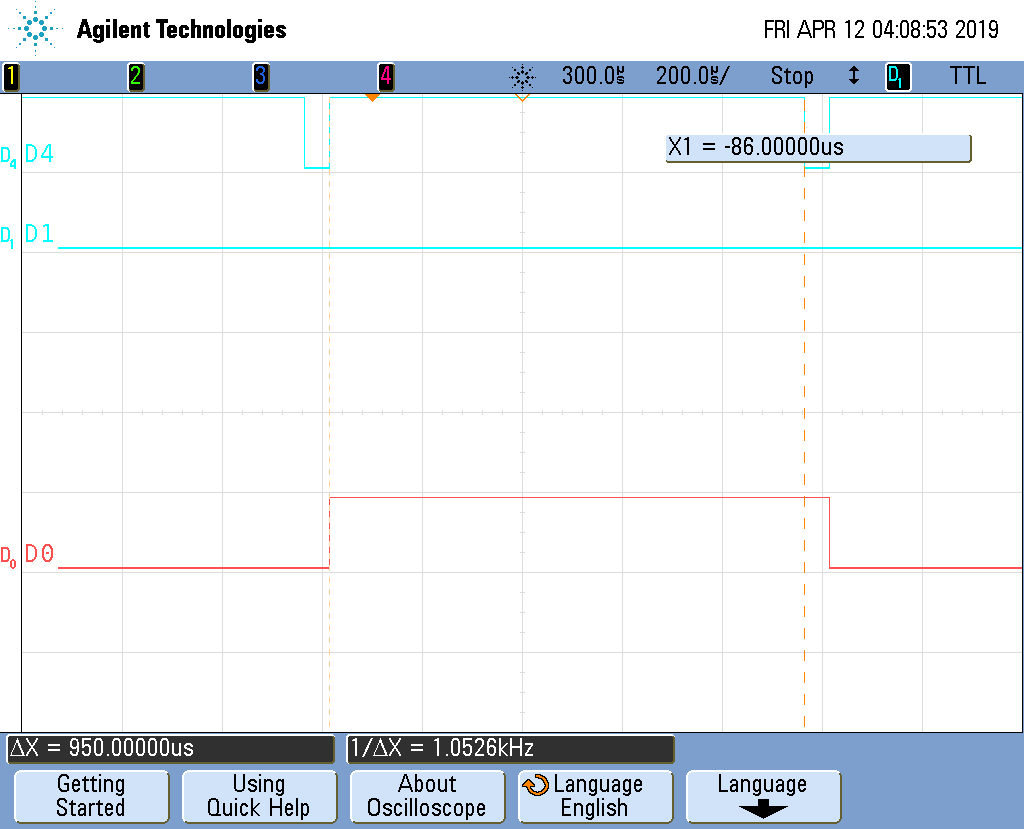
\includegraphics[width=.8\textwidth]{scope_11.png}
\caption{95\% Duty Cycle}
\label{fig:scope11}
\end{figure}
 
\section{Conclusion}
As an introductory lab to using the output compare module, this was a very effective lab. Designing an adjustable frequency PWM signal was surprisingly easy, and the information available made it all very easy. I've already used this information in my own projects where I used a PWM signal. As far as the relationship between generating a PWM signal and all of the uses of the output compare module, I do think the distinction is somewhat difficult to visualize. But that's somewhat due to the design of the peripheral itself.

As far as the relationship between the PWM cycle period and the PWM duty cycle resolution, the shorter the period of the PWM cycle / carrier period, the less fine your resolution will be. This is easy to visualize, if you're shortening the window of the PWM period (by increasing your frequency), then that smaller and smaller window can be subdivided into less resolute blocks of the timing mechanism. To take this to the extremes, a period which is constructed of only four clock cycles will only allow for 25\% resolution, as the very small cycle period is being divided into very few different 'blocks'. 

The output compare module has two different registers (a 'shadow' and a regualr one) that the user can interact with during initialization. However, after the output compare module is initialized, the second (non-shadow) register, cannot be accessed. The purpose of this is to prevent the PWM duty cycle from changing in the middle of one pulse width. Should the user change the value in the period register from 100\% to 0\% (not actual percentages but for the sake of explanation), while the output compare module was in the middle of a pulse, then the signal would drop early, resulting in an actual pulse width of neither 100\% or 0\%. The shadow register holds onto the user-loaded value for the compare module, but is only transferred into the actual comparison circuit when a given PWM period is completed; removing any extraneous results.

Although the output of the output compare module is strictly a digital signal, i.e. either 3.3V or GND, this can easily be turned into a continuous signal (such as a sinusoidal one) using circuitry. By passing the PWM wave through various combinations of resistors, capacitors, and inductors, a continuous signal can be created. In addition to this, there is also the option of simply having the PWM signal \textit{encode} a continuous signal that can be then be decoded by another process. Using a module like our output compare, the continuous signal would simply be converted to a digital value and then compared to an incrementing clock's digital value. This would result in the PWM output becoming a logical low whenever the clock signal exceeds the input signal, thus encoding the continuous input as a series of widths.

If I had changed \textbf{only} the prescale value for the timer, this would effectively double my PWM period. This is because it would now take the timer (N) times as long to reach the same period value, but with no increase in precision for this time. This is essentially like stretching the timer's signal over a longer period of time; resulting in worse resolution for the peripheral.

\end{document}